\documentclass{article}
\usepackage{setspace}
%\usepackage{subfigure}

\pagestyle{plain}
\usepackage{amssymb,graphicx,color}
\usepackage{amsfonts}
\usepackage{latexsym}
\usepackage{a4wide}
\usepackage{amsmath}
\usepackage{paper}
\usepackage{mathtools}

\newtheorem{theorem}{Theorem}
\newtheorem{lemma}[theorem]{Lemma}
\newtheorem{corollary}[theorem]{Corollary}
\newtheorem{proposition}[theorem]{Proposition}
\newtheorem{remark}[theorem]{Remark}
\newtheorem{definition}[theorem]{Definition}
\newtheorem{fact}[theorem]{Fact}

\newtheorem{problem}[theorem]{Problem}
\newtheorem{exercise}[theorem]{Exercise}
\def \set#1{\{#1\} }




\newenvironment{proof}{
PROOF:
\begin{quotation}}{
$\Box$ \end{quotation}}

\usepackage{xcolor}
\newcommand{\jk}[1]{{\color{blue} [JK: #1]}}
\newcommand{\jw}[1]{{\color{gray} [JW: #1]}}

\newcommand{\nats}{\mbox{\( \mathbb N \)}}
\newcommand{\rat}{\mbox{\(\mathbb Q\)}}
\newcommand{\rats}{\mbox{\(\mathbb Q\)}}
\newcommand{\reals}{\mbox{\(\mathbb R\)}}
\newcommand{\ints}{\mbox{\(\mathbb Z\)}}
\newcommand{\Cat}{\operatorname{\mathcal{C}}}
\newcommand{\Chol}{\operatorname{Chol}}
\newcommand{\KLD}{\operatorname{KLD}}
\newcommand{\tr}{\operatorname{tr}}
\newcommand{\diag}{\operatorname{diag}}
\newcommand{\GP}{\operatorname{\mathcal{GP}}}

\DeclareMathOperator*{\argmax}{arg\,max}
\DeclareMathOperator*{\argmin}{arg\,min}

% make sure equation numbers start with the section they are from
\numberwithin{equation}{section}
%%%%%%%%%%%%%%%%%%%%%%%%%%


\title{  	{ 
\includegraphics[scale=.5]{ucl_logo.png}}\\
{{\Huge Generalised Variational Inference for Sparse Gaussian Process Learning}}\\
{\large }\\
		}
\date{Submission date: September 2023}
\author{James Wu\thanks{
{\bf Disclaimer:}
This report is submitted as part requirement for the Master's in Computational Statistics \& Machine Learning Degree at UCL. It is
substantially the result of my own work except where explicitly indicated in the text.
\newline  %% \\ screws it up
\emph{Either: }The report may be freely copied and distributed provided the source is explicitly acknowledged
\newline  %% \\ screws it up
\emph{Or: }The report will be distributed to the internal and external examiners, but thereafter may not be copied or distrbuted except with permission from the author.}
\\ \\
Computational Statistics \& Machine Learning\\ \\
Supervisors: Veit Wild \& Jeremias Knoblauch}



\begin{document}

\onehalfspacing
\maketitle
\pagenumbering{gobble}
\newpage
\setcounter{page}{1}
\pagenumbering{roman}
\section*{Acknowledgements}
Thanks mom!
\newpage

\begin{abstract}
Summarise your report concisely.
\end{abstract}
\newpage
\tableofcontents
\newpage
\pagenumbering{arabic}
\setcounter{page}{1}
\section{GPs: Flexible but \textit{not} Scaleable}
Gaussian Processes (GPs) are powerful universal function approximators that can be used for both regression and classification tasks. In the following sections we will review GPs followed by a discussion of their strengths and weaknesses.
\subsection{The GP}\label{section:the-gp}
We introduce the GP following the formulation from \cite{rasmussen2003gaussian}. Given an input space $\mathcal{X}$, a GP is a random function mapping $F(\cdot)$ where a sample function $f(\cdot) \sim F(\cdot)$ applies the mapping $f: \mathcal{X} \rightarrow \mathbb{R}$. We denote:
\begin{align}
    f(\cdot) \sim F(\cdot) = \GP\left(m_p(\cdot), k_p(\cdot, \cdot)\right)
    \label{gp}
\end{align}
where a GP is defined with respect to a mean function $m_p: \mathcal{X} \rightarrow \mathbb{R}$ and a positive definite kernel function $k_p: \mathcal{X} \times \mathcal{X} \rightarrow \mathbb{R}$ such that:
\begin{align}
    F(\cdot) = \mathcal{N}(m_p(\cdot), k_p(\cdot, \cdot))
    \label{gp-normal}
\end{align}
In other words, for $N$ points $\mathbf{X}_N = \left\{ x_n\right\}_{n=1}^N$ where $x_n \in \mathcal{X}$, a GP constructs the Gaussian distribution for a random response vector $Y_N \in \mathbb{R}^{N}$:
\begin{align}
    \label{gp-vector}
    P\left(Y_N \vert \mathbf{X}_N\right) = F\left( \mathbf{X}_N\right) = \mathcal{N}\left(\mathbf{m}_{p\left(\mathbf{X}_N\right)}, \mathbf{K}_{p\left(\mathbf{X}_N, \mathbf{X}_N\right)}\right)
\end{align}
where $\mathbf{m}_{p(\mathbf{X}_N)} = \left[ m_p(x_1) \cdots m_p(x_N)\right]^T \in \mathbb{R}^N$ and $\mathbf{K}_{p(\mathbf{X}_N, \mathbf{X}_N)} \in \mathbb{R}^{N \times N}$ having elements:
\begin{align}
    \left[\mathbf{K}_{p(\mathbf{X}_N, \mathbf{X}_N)}\right]_{n, n'} = k_p(x_n, x_{n'})
\end{align}
for $n, n'=1,\dots, N$. Bold font $\mathbf{X}_N$ and $\mathbf{Y}_N$ will be a shorthand for denoting known vectors or matrices of the form $\mathbf{X}_N = \left\{ x_n\right\}_{n=1}^N$ and $\mathbf{Y}_N = \left\{ y_n\right\}_{n=1}^N$ respectively. $X_N$ and $Y_N$ will denote random vectors or matrices.
\subsection{GP Regression}
Consider the regression task where we have $N$ observation pairs $\left\{(x_n, y_n)\right\}_{n=1}^{N}$ with inputs $x_n \in \mathcal{X}$ and responses $y_n \in \mathbb{R}$. GP regression assumes the data generating process:
\begin{align}
    y_n \sim F(x_n) + E
    \label{regression-data-uncertainties}
\end{align}
where the GP random function mapping $F(\cdot)$ accounts for the epistemic (model) uncertainty and the random scalar $E$ accounts for the aleatoric (data) uncertainty. In this formulation, we assume that the aleatoric uncertainty is homoscedastic of the form:
\begin{align}
    E = \mathcal{N} \left(0, \sigma^2\right)
    \label{aleotric-uncertainty}
\end{align}
GP regression uses the formulation in Section~\ref{section:the-gp} to `predict' for $N^*$ test points $\mathbf{X}_{N^*} = \left\{ x_{n^*}\right\}_{n^*=1}^{N^*}$ with a Bayesian posterior. ($\ref{gp-vector}$) provides the prior for the response vector of the test points:
\begin{align}
    \label{gp-prior}
    P\left(Y_{N^*}\vert \mathbf{X}_{N^*}\right)
\end{align}
Evaluating the known training response vector $\mathbf{Y}_{N}$ provides the likelihood:
\begin{align}
     \label{gp-likelihood}
    P\left(\mathbf{Y}_{N} \vert Y_{N^*}, \mathbf{X}_{N^*}, \mathbf{X}_{N} \right)
\end{align}
With Bayes' Rule, the posterior of the response vector is proportional to the prior and likelihood:
\begin{align}
     P\left(Y_{N^*} | \mathbf{Y}_{N},  \mathbf{X}_{N},  \mathbf{X}_{N^*}\right) \propto P\left(\mathbf{Y}_{N} \vert Y_{N^*}, \mathbf{X}_{N^*}, \mathbf{X}_{N} \right) P\left(Y_{N^*}\vert \mathbf{X}_{N^*}\right)
    \label{bayes-posterior}
\end{align}
In GP regression, (\ref{bayes-posterior}) acts as a `prediction' for the epistemic uncertainty of the test point responses. With all terms being Gaussian, the posterior in (\ref{bayes-posterior}) has the form:
\begin{align}
    P\left(Y_{N^*} | \mathbf{Y}_{N},  \mathbf{X}_{N},  \mathbf{X}_{N^*}\right)  =  \mathcal{N}\left(\hat{\mathbf{m}}_{p(\mathbf{X}_{N^*})}, \hat{\mathbf{K}}_{p(\mathbf{X}_{N^*}, \mathbf{X}_{N^*})}\right)
    \label{gp-epistemic-posterior}
\end{align}
with:
\begin{align}
    \label{gp-epistemic-posterior-mean}
    \hat{\mathbf{m}}_{p(\mathbf{X}_{N*})} = \mathbf{m}_{p(\mathbf{X}_{N*})} + \mathbf{K}_{p(\mathbf{X}_{N*}, \mathbf{X}_N)} \mathbf{K}_{p(\mathbf{X}_N, \mathbf{X}_N)}^{-1} \left( \mathbf{Y}_N - \mathbf{m}_{p(\mathbf{X}_N)}\right)
\end{align}
and
\begin{align}
    \label{gp-epistemic-posterior-covariance}
    \hat{\mathbf{K}}_{p(\mathbf{X}_{N*}, \mathbf{X}_{N*})} = \mathbf{K}_{p(\mathbf{X}_{N*}, \mathbf{X}_{N*})} - \mathbf{K}_{p(\mathbf{X}_{N*}, \mathbf{X}_N)}\mathbf{K}_{p(\mathbf{X}_N, \mathbf{X}_N)}^{-1}\mathbf{K}_{p(\mathbf{X}_N, \mathbf{X}_{N*})}
\end{align}
With the aleoteric data uncertainty also modelled as a Gaussian in (\ref{aleotric-uncertainty}), GP regression models the test data responses in the closed form:
\begin{align}
    \mathbf{Y}_{N^*} \sim P_{\GP}\left(Y_{N^*} \vert \mathbf{Y}_N, \mathbf{X}_N, \mathbf{X}_{N^*}, \sigma^2\right)
    \label{gp-posterior}
\end{align}
This is known as the predictive posterior where:
\begin{align}
    P_{\GP}\left(Y_{N^*} \vert \mathbf{Y}_N, \mathbf{X}_N, \mathbf{X}_{N^*}, \sigma^2\right) = \mathcal{N}\left(\bar{\mathbf{m}}_{p(\mathbf{X}_{N^*})}, \bar{\mathbf{K}}_{p(\mathbf{X}_{N^*}, \mathbf{X}_{N^*})}\right)
    \label{gp-posterior-normal}
\end{align}
with:
\begin{align}
    \label{gp-posterior-mean}
    \bar{\mathbf{m}}_{p(\mathbf{X}_{N*})} = \mathbf{m}_{p(\mathbf{X}_{N*})} + \mathbf{K}_{p(\mathbf{X}_{N*}, \mathbf{X}_N)} \left( \mathbf{K}_{p(\mathbf{X}_N, \mathbf{X}_N)} + \sigma^2 \mathbf{I}_N\right)^{-1} \left( \mathbf{Y}_N - \mathbf{m}_{p(\mathbf{X}_N)}\right)
\end{align}
and
\begin{align}
    \label{gp-posterior-covariance}
    \bar{\mathbf{K}}_{p(\mathbf{X}_{N*}, \mathbf{X}_{N*})} = \mathbf{K}_{p(\mathbf{X}_{N*}, \mathbf{X}_{N*})} - \mathbf{K}_{p(\mathbf{X}_{N*}, \mathbf{X}_N)}\left( \mathbf{K}_{p(\mathbf{X}_N, \mathbf{X}_N)} + \sigma^2 \mathbf{I}_N\right)^{-1}\mathbf{K}_{p(\mathbf{X}_N, \mathbf{X}_{N*})}
\end{align}
where $\mathbf{I}_N \in \mathbb{R}^{N \times N}$ is the identity matrix.

\subsection{GP Classification}
% \subsubsection{Binary Classification}
% For binary GP classification, a mapping is defined:
% \begin{align}
% g: \mathbb{R} \rightarrow [0, 1]
% \end{align}
% transforming a value on the real line to the unit interval to represent a probability.
% A Bernoulli random variable $\mathcal{B}$ can be defined such that:
% \begin{align}
% F_c \sim \mathcal{B}(g(F))
% \end{align}
% where $F_c \in \{0, 1\}$ is a random vector, providing the desired binary classifier behaviour.
% \subsubsection{Multi-label Classification}
Consider the classification task where we have $N$ observation pairs $\left\{(x_n, y_n)\right\}_{n=1}^{N}$ with inputs $x_n \in \mathcal{X}$ and responses $y_n \in \{1, \dots, J\}$. In other words, each input $x$ is mapped to one of $J$ labels. Following the GP classification approach from \cite{matthews2017scalable}, we first construct a GP regression model for each label such that for a test point $x \in \mathcal{X}$, the posterior prediction is Gaussian:
\begin{align}
    y^j \sim \mathcal{N}\left(\bar{m}_p^j(x), \bar{k}_p^j(x, x)\right)
    \label{gp-classifier-regressors}
\end{align}
where $j=1, \dots, J$, defining $J$ i.i.d. random vectors from $J$ i.i.d GPs.
Concatenating $\mathbf{y}^{1:J} = [y^1 \cdots y^J]^T \in \mathbb{R}^{J}$, this real-valued vector is mapped to one of $J$ labels through a series of operations to the GP classifier:
\begin{align}
y \sim \Cat \left(s\left(\mathbf{y}^{1:J}\right)\right)
\label{gp-classifier}
\end{align}
where $y \in \{1, \dots, J\}$, the desired label response. This approach requires defining $s: \mathbb{R}^J \rightarrow \Delta(J)$, a mapping from a $J$ dimensional real vector to a $J$ dimensional probability simplex $\Delta(J)$ which is used to parameterise a categorical distribution $\Cat$ (a generalisation of the Bernoulli distribution to $J$ labels).

\subsubsection{The Robust Max Function}
The formulation in (\ref{gp-classifier}) requires defining a mapping $s: \mathbb{R}^J \rightarrow \Delta(J)$. \cite{matthews2017scalable} provides a few differen choices for $s$. Following \cite{wild2022generalized}, we will use the robust max function, defining the $j^{th}$ element of the probability simplex:
\begin{align}
s_{j, robust}^{(\epsilon)}\left(\mathbf{y}^{1:J}\right) = \begin{cases}
      1-\epsilon, &  \text{if } j = \arg \max\left(\mathbf{y}^{1:J}\right) \\
      \frac{\epsilon}{J-1}, & \text{otherwise} \\
   \end{cases}
   \label{robust-max-function}
\end{align}
where $\epsilon \in [0, 1]$. Practically, $\epsilon$ is a very small value (i.e. $1e^{-2}$). Constructing the $\Delta(J)$ vector with (\ref{robust-max-function}), we have the probability value of $1-\epsilon$ for the label of maximum value and $\frac{\epsilon}{J-1}$ otherwise. This formulation provides robustness to outliers, as it only considers the ranking of the GP models for each label.
\\A benefit of the robust max function is that the expected log-likelihood under $P$, the categorical distribution in (\ref{gp-classifier}), becomes analytically tractable. \cite{wild2022generalized} shows that with $N$ input and response pairs $\{x_n, y_n\}_{n=1}^N$:
\begin{align}
    \mathbb{E}_{P} \left[\log p\left(y \vert y^{1:J}\right)\right] \approx \sum_{n=1}^N \log(1-\epsilon) S_p(x_n, y_n) + \log\left(\frac{\epsilon}{J-1}\right) \left(1-S_p(x_n, y_n)\right)
    \label{robust-max-function-expected-log-likelihood}
\end{align}
with:
\begin{align}
    S_p(x_n, j) \coloneqq \frac{1}{\sqrt{\pi}}\sum_{i=1}^{I} w_i \left(\prod_{j'=1, j'\neq j}^J \phi\left(\frac{\xi_i\sqrt{(2 \bar{k}^{j'}_p(x_n, x_n)}+\bar{m}^{j}_p(x_n) - \bar{m}^{j'}_p(x_n)}{\sqrt{\bar{k}^{j'}_p(x_n, x_n)}}\right)\right)
\end{align}
where $\left\{w_i, \xi_i\right\}_{i=1}^I$ are the weights and roots of the Hermite polynomial of order $I \in \mathbb{N}$ and  $\phi(\cdot)$ is the standard normal cumulative distribution function. This analytical expression can be used for inference on GP classifier parameters when defining a loss objective with respect to the log-likelihood.

\subsection{The GP Lacks Scaleability}
In both regression and classification tasks, GPs are an extremely flexible modelling approach. Minimal requirements on the mean function $m_p: \mathcal{X} \rightarrow \mathbb{R}$ and postive definite kernel function $k_p: \mathcal{X} \times \mathcal{X} \rightarrow \mathbb{R}$ in (\ref{gp}) provide endless choices for GP construction. This offers complete control and visibility into the model's behaviour, a strong advantage compared to other modelling approaches. 

The main drawback of GPs has been their inability to scale with respect to $N$, the number of training points. Both classification and regression relies on evaluating the inversion of an $\mathbb{R}^{N \times N}$ matrix in $\ref{gp-posterior-mean}$ and $\ref{gp-posterior-covariance}$. This operation has computational complexity $\mathcal{O}(N^3)$ and space complexity $\mathcal{O}(N^2)$, both of which quickly become problematic when scaling to larger-sized training sets. Despite their impressive performance and theoretically-driven Bayesian approach, the computational intractability of GPs has been a serious limitation, restricting their application to problem domains with smaller sized training data sets. In the next section, we will present sparse variational Gaussian Processes (svGPs), a common approach to scaling GPs to larger data sets.


\newpage
\section{svGPs: Scaleable but \textit{not} Flexible}
Sparse variational Gaussian Processes (svGPs) proposed by \cite{titsias2009variational}, are a common approach to ensuring computational tractability when scaling GPs. We will review this formulation followed by a discussion of the strengths and weakness of the approach.

\subsection{The svGP}
The svGP assumes that a subset of inducing points $\{x_m, y_m\}_{m=1}^{M} \subset \{x_n, y_n\}_{n=1}^{N}$ where $M << N$ can adequately capture the relationships in the full training data. This approach constructs an svGP:
\begin{align}
g(\cdot) \sim \GP\left(m_q^{(\nu)}(\cdot), k_q^{(\nu)}(\cdot, \cdot)\right)
\label{svgp}
\end{align}
parameterised by $\nu$ which includes the choice of subset $\{x_m, y_m\}_{m=1}^{M}$ and has $\mathcal{O}(M^3)$ predictive computational complexity. For $N^*$ test points $\mathbf{X}_{N^*}$, the svGP has an approximate predictive posterior:
\begin{align}
    \mathbf{Y}_{N^*} \sim Q_{\GP}^{(\nu)}\left(Y_{N^*} \vert \mathbf{X}_{N^*}\right)
\end{align}
where:
\begin{align}
    Q_{\GP}^{(\nu)}\left(Y_{N^*} \vert \mathbf{X}_{N^*}\right) = \mathcal{N}\left(\bar{\mathbf{m}}_{q\left(\mathbf{X}_{N^*}\right)}^{(\nu)}, \bar{\mathbf{K}}_{q\left(\mathbf{X}_{N^*}, \mathbf{X}_{N^*}\right)}^{(\nu)}\right)
\end{align}
\cite{titsias2009variational} proposes formulating the approximate predictive posterior mean function parameterised by a vector $\boldsymbol{\mu} \in \mathbb{R}^M$:
\begin{align}
    \label{svgp-mean} 
    \bar{\mathbf{m}}_{q\left(\mathbf{X}_{N^*}\right)}^{(\nu)} = \mathbf{m}_{p\left(\mathbf{X}_{N^*}\right)} +  \mathbf{K}_{p( \mathbf{X}_{N^*}, \mathbf{X}_M)}\mathbf{K}_{p(\mathbf{X}_M, \mathbf{X}_M)}^{-1} \boldsymbol{\mu}
\end{align}
where $\mathbf{X}_M = \left\{ x_m\right\}_{m=1}^M$ and a kernel function parameterised by a positive definite matrix $\mathbf{\Sigma} \in \mathbb{R}^{M\times M}_{\succ 0}$:
% \begin{multline}
% \begin{split}
% \bar{\mathbf{K}}_{q\left(\mathbf{X}_{N^*}, \mathbf{X}_{N^*}\right)}^{(\nu)} &=  \mathbf{K}_{p\left(\mathbf{X}_{N^*}, \mathbf{X}_{N^*}\right)} \\
% & - \mathbf{K}_{p(\mathbf{X}_{N^*}, \mathbf{X}_M)} \mathbf{K}_{p(\mathbf{X}_M, \mathbf{X}_M)}^{-1}\mathbf{K}_{p(\mathbf{X}_M, \mathbf{X}_{N^*})} \\
% & + \mathbf{K}_{p(\mathbf{X}_{N^*}, \mathbf{X}_M)}  \mathbf{K}_{p(\mathbf{X}_M, \mathbf{X}_M)}  ^{-1} \mathbf{\Sigma}\mathbf{K}_{p(\mathbf{X}_M, \mathbf{X}_M)}^{-1} \mathbf{K}_{p(\mathbf{X}_M, \mathbf{X}_{N^*})}
% \end{split}
% \label{svgp-covariance}
% \end{multline}
\begin{align}
\bar{\mathbf{K}}_{q\left(\mathbf{X}_{N^*}, \mathbf{X}_{N^*}\right)}^{(\nu)} & = \mathbf{K}_{p\left(\mathbf{X}_{N^*}, \mathbf{X}_{N^*}\right)} \nonumber \\
&\qquad - \mathbf{K}_{p(\mathbf{X}_{N^*}, \mathbf{X}_M)} \mathbf{K}_{p(\mathbf{X}_M, \mathbf{X}_M)}^{-1}\mathbf{K}_{p(\mathbf{X}_M, \mathbf{X}_{N^*})} \nonumber \\
&\qquad + \mathbf{K}_{p(\mathbf{X}_{N^*}, \mathbf{X}_M)}  \mathbf{K}_{p(\mathbf{X}_M, \mathbf{X}_M)}  ^{-1} \mathbf{\Sigma}\mathbf{K}_{p(\mathbf{X}_M, \mathbf{X}_M)}^{-1} \mathbf{K}_{p(\mathbf{X}_M, \mathbf{X}_{N^*})}
\label{svgp-covariance}
\end{align}
Together, these define the parameter space:
\begin{align}
    \mathbf{\Gamma} = \left\{\boldsymbol{\mu} \in \mathbb{R}^{M}, \mathbf{\Sigma} \in \mathbb{R}^{M\times M}_{\succ 0}, \left\{x_m, y_m\right\}_{m=1}^{M} \subset \{x_n, y_n\}_{n=1}^{N}\right\}
    \label{svgp-parameter-space}
\end{align}
We wish to find $\nu^* \in \Gamma$ such that for any test points $\mathbf{X}_{N^*}$ the svGP Gaussian distribution $Q^{(\nu^*)}$ approximates the exact posterior distribution from ($\ref{bayes-posterior}$):
\begin{align}
    P_{\GP}\left(Y_{N^*} \vert \mathbf{X}_{N^*}, \mathbf{Y}_N, \mathbf{X}_N, \sigma^2 \right) \approx Q_{\GP}^{(\nu^*)}\left(Y_{N^*} \vert \mathbf{X}_{N^*}\right)
    \label{svgp-desired-approximation}
\end{align}
To approximate the exact predictive posterior, \cite{titsias2009variational} derives the free energy lower bound:
\begin{align}
    math
    \label{elbo}
\end{align}
Thus, the approximation in (\ref{svgp-desired-approximation}) is equivalent to minimising the KL-divergence:
\begin{align}
    \nu^* = \argmin_{\nu \in \Gamma}\KLD \left[ Q_{\GP}^{(\nu)}\left(Y_{N^*} \vert \mathbf{X}_{N^*}\right) \Big\| P_{\GP}\left(Y_{N^*} \vert \mathbf{X}_{N^*}, \mathbf{Y}_N, \mathbf{X}_N, \sigma^2 \right) \right]
\end{align}
for any test points $\mathbf{X}_{N^*}$. \cite{titsias2009variational} shows that for a given set of inducing points $\left\{ x_m, y_m\right\}_{m=1}^M$, the optimal choices $\boldsymbol{\mu}^*$ and $\mathbf{\Sigma}^*$ have the closed forms:
\begin{align}
    \label{svgp-optimal-mean}
    \boldsymbol{\mu}^* = \sigma^{-2}\mathbf{K}_{p(\mathbf{X}_M, \mathbf{X}_M)} \left( \mathbf{K}_{p(\mathbf{X}_M, \mathbf{X}_M)} + \sigma^{-2}\mathbf{K}_{p(\mathbf{X}_M, \mathbf{X}_N)}\mathbf{K}_{p(\mathbf{X}_N, \mathbf{X}_M)}\right)^{-1}\mathbf{K}_{p(\mathbf{X}_M, \mathbf{X}_N)} \left(\mathbf{Y}_N - \mathbf{m}_{p\left(\mathbf{X}_N\right)}\right)
\end{align}
and
\begin{align}
    \label{svgp-optimal-covariance}
    \mathbf{\Sigma}^* = \mathbf{K}_{p(\mathbf{X}_M, \mathbf{X}_M)} \left(\mathbf{K}_{p(\mathbf{X}_M, \mathbf{X}_M)} +  \sigma^{-2}\mathbf{K}_{p(\mathbf{X}_M, \mathbf{X}_N)}\mathbf{K}_{p(\mathbf{X}_N, \mathbf{X}_M)}\right)^{-1}\mathbf{K}_{p(\mathbf{X}_M, \mathbf{X}_M)}
\end{align}
This formulation ensures matrix inversion of matrices of $\mathbb{R}^{M \times M}$ with $\mathcal{O}\left(M^3\right)$ computational complexity. The operation $\mathbf{K}_{p(\mathbf{X}_M, \mathbf{X}_N)}\mathbf{K}_{p(\mathbf{X}_N, \mathbf{X}_M)}$ in (\ref{svgp-optimal-mean}) and (\ref{svgp-optimal-covariance}) has computational complexity $\mathcal{O}\left(NM^2\right)$, but is a pre-computed constant. Thus, the predictive computational complexity of this approach is $\mathcal{O}\left(M^3\right)$ with space complexity is $\mathcal{O}\left(M^2\right)$, significantly improving the scalability of GP approaches.

\subsubsection{Inducing Points Selection}
Finding the optimal inducing points $\left\{x_m, y_m\right\}_{m=1}^{M} \subset \{x_n, y_n\}_{n=1}^{N}$ that optimise the loss objective $\mathcal{L}(\nu)$ in ($\ref{elbo}$) can be computationally expensive. \cite{burt2020convergence} proposes a greedy variance selection method which iteratively selects the next inducing point based on the highest marginal variance in the prior conditioned on the current set of inducing points:
\begin{align}
    \label{greedy-varaince-selection}
    \text{index}_{m+1} = \argmax \left(\diag \left(\mathbf{K}_{p(\mathbf{X}_N, \mathbf{X}_N)} - \mathbf{K}_{p(\mathbf{X}_N, \mathbf{X}_{m})} \mathbf{K}_{p(\mathbf{X}_{m}, \mathbf{X}_{m})}^{-1}\mathbf{K}_{p(\mathbf{X}_{m}, \mathbf{X}_N)}\right)\right)
\end{align}
where $m < M$, $\mathbf{X}_{m}$ are the $m$ inducing points already chosen, and $\text{index}_{m+1}$ is the index of the next inducing point.

\subsection{The svGP Lacks Flexibility}
The svGP from \cite{titsias2009variational} provides a solution to the scaling issues of the GP but comes with with an unfortunate drawback. The mean and kernel functions must conform to the formulations of (\ref{svgp-mean}) and (\ref{svgp-covariance}) respectively. Although svGPs are more scaleable, they have lost the powerful modelling flexibility of the GP. In the following sections, we will better understand the reasons for the restrictive mean and kernel function formulations of the svGP. This will include reviewing the link between GPs and Gaussian measures (GMs) on function spaces and the mis-match of support problem of the KL-divergence for Gaussian measures on function spaces. 

\subsubsection{The Kolomogorov Extension Theorem}
A GP is guaranteed to have at least one GM formulations on a function space. To better understand this, we first review the Kolmogorov Extension Theorem:
\begin{theorem}[Kolmogorov Extension Theorem]
\label{kolomogorov-extension-theorem}
Given a finite space measure such that:
\begin{align}
    consistency 
    \label{kolomogorov-consistency}
\end{align}
Then there exists a probability measure on the product sigma algebra ... 
\begin{align}
    measure
    \label{kolomogorov-measure}
\end{align}
In other words, consistency guarantees the existence of a corresponding measure on a function space.
\end{theorem}
From (\ref{gp-vector}), we see that a GP will always generate a set of points which conform to a Gaussian distribution, satisfying the consistency condition of (\ref{kolomogorov-consistency}). As such, the Kolmogorov Extension Theorem guarantees the existence of at least one GM corresponding to this GP in some measureable function space. 

\subsubsection{The Kullback-Leibler Divergence in Function Spaces}
The existence of corresponding GM guaranteed by the Kolomogorov Extension Theorem can be trivially constructed over the space of all functions $\mathcal{F} = \left\{f: \mathbb{R}^{N} \rightarrow \mathbb{R} \right\}$. Without other assumptions on the GP construction, we can't ensure the existence of a corresponding GM on a more well-behaved function space. Thus, (\ref{elbo}) requires a KL-divergence on the function space $\mathcal{F}$:
\begin{align}
    \label{kld-function-spaces}
\end{align}
\cite{matthews2016sparse} shows that ensuring a valid KL divergence on $\mathcal{F}$ requires maintaining the existence of the Radon-Nikodym derivative:
\begin{align}
\frac{dQ^{\nu}}{d P^{F \vert \mathbf{Y}_N}}
\label{radon-nikodym}
\end{align}
\cite{matthews2016sparse} explains that the strict svGP formulation of (\ref{svgp-optimal-mean}) and (\ref{svgp-optimal-covariance}) from \cite{titsias2009variational} are necessary to ensure the existence of the Radon-Nikodym derivative in (\ref{radon-nikodym}). In other words, the svGP has limited flexibility due to the problem of support mis-match for the KL-divergence on $\mathcal{F}$.

\subsubsection{Approximation Approaches}
\jw{existing approaches to approximate the KL divergence kinda work but dont get to the core problem of the KL divergence. We will show in the next section that the KL divergence is a result of the Bayesian posterior approach}
\subsubsection{The Bayesian Posterior}
\\\jw{Explain that we get the KL from our Bayesian approach. Thus the problem of kl-divergence support mismatch can be traces to the bayesian variational inference approach. This motivate the generalised Bayes approach that we will introduce in the next section, which will provide a way to get rid of the KL, freeing us from the support mismatch problem}
In a Bayesian context (see section \ref{svgp-kld-bayesian} for more details), this involves minimisation of the Kullback-Leibler (KL) divergence:
\begin{align}
    \nu^* = \argmin_{\nu \in \Gamma} \KLD\left(Q^\nu\left(\mathbf{Y}_{N*} \Big\vert \left\{ x_{n*}\right\}_{n*=1}^{N*}\right) \Big\| P\left(\mathbf{Y}_{N*} \Big\vert \left\{ y_n\right\}_{n=1}^N,  \left\{ x_n\right\}_{n=1}^N,  \left\{ x_{n*}\right\}_{n*=1}^{N*}\right) \right)
    \label{svgp-minimiser}
\end{align}
where $\Gamma$ is the parameterisation set for the svGP and the KL divergence is defined as:
\begin{align}
    \KLD\left(Q^{\nu} \Big\| P^{F \vert \mathbf{Y}_N} \right) = \int \log \left( \frac{dQ^{\nu}}{d P^{F \vert \mathbf{Y}_N}} \right) d Q^{\nu}(f)
    \label{svgp-kld-loss}
\end{align}
where $P^{F \vert \mathbf{Y}_N}$ denotes the posterior distribution of $GP(m_p, k_p)$.


For the posterior and approximation to exhibit the same behaviour requires an optimisation process on $\nu$.
\\To ensure the existence of the Radon-Nikodym derivative $\frac{dQ^{\nu}}{d P^{F \vert \mathbf{Y}_N}}$, \cite{matthews2016sparse} and \cite{titsias2009variational} show that (\ref{svgp-kld-loss}) is a valid expression when $Q_{GP}^{\nu}$ is defined in a very specific fashion. 
\\The formulation above defines a Gaussian Process with a matrix inversion operation of $\mathcal{O}(M^3)$, providing us a computationally tractable approach. Moreover, the parameterisation set $\Gamma$ is defined:
\begin{align}
    \Gamma = \left\{\mathbf{\mu} \in \mathbb{R}^{M}, \mathbf{\Sigma} \in \mathbb{R}^{M\times M}_{\succ 0}, \left\{x_m, y_m\right\}_{m=1}^{M} \subset \{x_n, y_n\}_{n=1}^{N}\right\}
    \label{svgp-parameter-set}
\end{align}
It is shown in \cite{matthews2016sparse} that:
\begin{align}
    \KLD\left(Q_{GP}^{\nu} \Big\| P_{GP}^{F \vert \mathbf{Y}_N} \right) = \sum_{n=1}^N\log p(y_n) - \mathcal{L}(\nu)
    \label{svgp-kld-loss-equivalence}
\end{align}
where $p(y_n)$ is the marginal likelihood or evidence of observing $yx_n$ under the prior $F_P \sim GP(m_p, k_p)$ and observation model $y_n \sim \mathcal{N}(F_P(x_i), \sigma^2)$ with $\sigma^2$ being the aleoteric uncertainty. $\mathcal{L}(\nu)$ is the variational free energy:
\begin{align}
    \mathcal{L}(\nu) = \mathbb{E}_{F_Q \sim Q_{GP}^{\nu}}\left[\sum_{n=1}^{N}\log p\left(y_n \vert \mu=F_Q(x_n), \sigma^2\right)\right] -\KLD\left(Q^{\nu}_{GP}\Big\| P_{GP}\right)
\end{align}
also referred to as the evidence lower bound (ELBO).
\\We see from (\ref{svgp-kld-loss-equivalence}) that $\mathcal{L}(\nu)$ is the only dependence on $\nu$, so we can rewrite our minimisation objective in (\ref{svgp-minimiser}):
\begin{align}
    \nu^* = \argmin_{\nu \in \Gamma} \left\{\mathbb{E}_{F_Q \sim Q^{\nu}}\left[\sum_{n=1}^{N}\log p\left(y_n \vert \mu=F_Q(x_n), \sigma^2\right)\right] -\KLD\left(Q^{\nu}_{GP}\Big\| P_{GP}\right)\right\}
    \label{svgp-minimiser-gvi-kld}
\end{align}
Moreover, the lower bound objective in ($\ref{elbo}$) will have the form:
\begin{align}
    \label{svgp-optimal-elbo}
    \mathcal{L}(\nu^*) = &-\frac{N}{2} \log\left(2\pi \right)\\
    &-\frac{1}{2} \log \left(\det\left( \mathbf{K}_{\mathbf{X}_N, \mathbf{X}_M}\left(\mathbf{K}_{\mathbf{X}_M, \mathbf{X}_M}\right)^{-1} \mathbf{K}_{\mathbf{X}_M, \mathbf{X}_N}\right)\right)\\
    & -\frac{1}{2} \left(\mathbf{Y}_N\right)^T \left( \mathbf{K}_{\mathbf{X}_N, \mathbf{X}_M}\left(\mathbf{K}_{\mathbf{X}_M, \mathbf{X}_M}\right)^{-1} \mathbf{K}_{\mathbf{X}_M, \mathbf{X}_N}\right)^{-1} \mathbf{Y}_N \\
    &  - \frac{1}{2\sigma^2}\tr\left(\mathbf{K}_{\mathbf{X}_N, \mathbf{X}_N} - \mathbf{K}_{\mathbf{X}_N, \mathbf{X}_M}\left(\mathbf{K}_{\mathbf{X}_M, \mathbf{X}_M}\right)^{-1} \mathbf{K}_{\mathbf{X}_M, \mathbf{X}_N}\right)
\end{align}
where we assume an optimal selection of inducing points $\left\{x_m, y_m\right\}_{m=1}^{M} \subset \{x_n, y_n\}_{n=1}^{N}$.
\\It is important to note that the existence of the objectives in (\ref{svgp-minimiser}) and (\ref{svgp-minimiser-gvi-kld}) \textit{requires} $P_{GP}^{F \vert \mathbf{Y}_N}$ to dominate $Q_{GP}^{\nu}$, which is \textit{only} guaranteed under the specific formulation of $Q$ in ($\ref{svgp-mean}$) and ($\ref{svgp-covariance}$). This severely restricts our choices for $m_q$ and $k_q$.


% Often lots of citations here (and elsewhere), e.g. \cite{Rey:D} or \cite[Theorem 2.3]{PriorNOP70}.   Bibtex can help with this, but is not essential. If you want pictures, try

% \begin{center}
% \includegraphics[scale=.5]{aristotle.jpg}
% \end{center}
% You can use
% \begin{itemize}
% \item lists
% \item like this
% \end{itemize}
% or numbered
% \begin{enumerate}
% \item like this,
% \item or this
% \end{enumerate}
% but don't overdo it.

% \section{Bayesian Variational Inference restricts svGP's}
% If you have a formal theorem you might try this.
% \begin{definition}\label{def}
% See definition~\ref{def}.
% \end{definition}
% \begin{theorem}
% For all $n\in\nats,\; 1^n=1$.
% \end{theorem}
% \begin{proof}
% By induction over $n$.
% \end{proof}
\newpage
\section{Generalised Variational Inference (GVI) for GPs}
\subsection{Generalising the Bayesian Posterior}
Statistical modelling is traditionally focused on characterising an underlying data generation process. In a Bayesian context, this involves updating the beliefs on a model's parameterisation. Given a model parameterised by $\theta$, Bayesian inference can be viewed as an update rule on $\pi(\theta)$, the prior belief of $\theta$. For new observations $x_{1:N}$ and a likelihood function $p(x_{1:N}|\theta)$, the belief for $\theta$ is updated as:
\begin{align}
q_B^*(\theta) = \frac{p(x_{1:N}|\theta) \pi(\theta)}{\int_{\Theta} p(x_{1:N}|\theta) d \pi(\theta)}
\label{bayesian-posterior}
\end{align}
where $q_B^*(\theta)$ is known as the \textit{Bayesian posterior}. The validity of the Bayesian Posterior relies on three assumptions concerning the prior, the likelihood, and the normaliser. In contrast to traditional statistical modelling, larger-scaled models like Bayesian Neural Networks are typically focused on \textit{predictive performance} rather than \textit{model specification}. In these settings, the three  assumptions for the Bayesian posterior quickly breakdown, making it no longer reasonable to view $q_B^*(\theta)$ as a Bayesian belief update.

\subsubsection{The Bayesian Posterior Interpretation Breaks Down}
Bayesian inference assumes a prior $\pi(\theta)$ that is well-specified and informative of $\theta^*$, the `true' model parameters. The prior is interpreted as embodying \textit{all} previous knowledge about the data generating process such as previously observed data. Alternatively, the prior can also be interpreted as representing \textit{pseudo} observations about how we believe the data behaves.Larger-scaled models are often over-parameterised black box models, such as the weights of a Bayesian neural network. These parameters are essentially uninterpretable and priors are chosen out of convenience (i.e. Gaussians) with little thought given to their true parameterisation. In these settings, it is no longer practical to view $\pi(\theta)$ as a prior belief in the parameters of the data generating model as it is most definitely mis-specified.
\\Bayesian inference assumes that there exists $\theta^* \in \Theta$, such that $x_i \sim p(x_n | \theta^*)$ for some unknown but fixed $\theta^*$. In other words $p(x_n | \theta^*)$, the likelihood function that is chosen is \textit{exactly} the true data generating process and is parameterised by $\theta$. In this case, the problem is simply a matter of finding $\theta^*$. Although model mis-specification occurs in traditional Bayesian inference, techniques such as hypothesis testing, residual analysis, and domain expertise can help guide the construction of a reasonably well-specified setting. However, the intentions behind using larger-scaled models is completely different. It is not to \textit{understand} the data generating process, but rather to have superior \textit{predictive performance}. With over-parameterisation, these black box models are most definitely mis-specified but often provide high prediction accuracy. As such, model parameters are typically chosen through an optimisation process (i.e. gradient descent), no longer adhering to the spirit of traditional Bayesian inference. For larger-scaled models, it is almost never fair to assume that $x_n \sim p(x|\theta)$ for \textit{any} $\theta \in \Theta$.
\\Bayesian inference assumes that the normaliser $\int_{\Theta} p(x_{1:N}|\theta) d \pi(\theta)$ is a tractable integral or is computationally tractable. Computational tractability assumes access to  adequate computational resources and time to reasonably approximate the integral. This means that in traditional Bayesian inference, the computational complexities of evaluating $q_B^*(\theta)$ can be ignored. The use of conjugate priors is the only case when there exists closed form expressions for $\int_{\Theta} p(x_{1:N}|\theta) d \pi(\theta)$ to ensure tractable evaluation of $q_B^*(\theta)$. For over-parameterised black-box models, $q_B^*(\theta)$ will need to be approximated either through sampling approximations of the normaliser or variational approximations of $q_B^*(\theta)$.
\newline
\\Samplers such as Metropolis Hastings or Markov Chain Monte Carlo only have convergence guarantees in the infinite limit. For small/moderately sized models, large enough samples will practically converge to the desired posterior. However, larger-scaled models generally require access to much more computational resources and time that is often impractical.
\newline
\\Approximating $q_B^*(\theta)$ involves solving for $q_A^*(\theta) \in \mathcal{Q}_{A}$, where $\mathcal{Q}_{A}$ is often viewed as distributions of a simpler form. For example mean field approximations define a family of distributions $\mathcal{Q}_{MF} = \left\{\prod_i q_i(\theta_i)\right\}$, a product of independent distributions. Variational inference is motivated to finding a $q_A^*(\theta) \in \mathcal{Q}_{A}$ that \textit{approximates} $q_B^*(\theta)$, through the minimisation of some divergence between the two, $D(q_A^*(\theta)\| q_B^*(\theta))$. However the space of distributions $\mathcal{Q}_{A}$ is usually severely restrictive in its expressiveness and $q_A^*(\theta)$ is almost never a fair depiction of the structure of $q_B^*(\theta)$. Realistically, $\mathcal{Q}_{A}$ is chosen purely for computational convenience. With larger-scaled models, it is often no longer reasonable to assume that the normaliser of the Bayesian posterior will be tractable or that $q_B^*(\theta)$ can be reasonably approximated in a tractable manner.

\subsubsection{The Generalised Posterior}
Interpreting the mechanism behind calculating the Bayesian posterior in the context of optimisation can provide a more reasonable depiction of $q_B^*(\theta)$ for larger-scaled models. It can be shown that $q_B^*(\theta)$ solves a special case of a general variational inference (GVI) problem:
\begin{align}
q^*(\theta) = \argmin_{q \in \Pi} \left\{ \mathbb{E}_{q(\theta)}\left[\frac{1}{N}\sum_{n=1}^N \ell(\theta, x_n)\right] + D(q\|\pi)\right\}
\label{general-posterior}
\end{align}
where $q_B^*(\theta)$ is recovered by choosing the negative log-likelihood loss $\ell(\theta, \cdot) = -\log p(\cdot | \theta)$, the Kullback-Leibler divergence $D(\cdot \| \pi) = \KLD(\cdot \| \pi)$, and the feasible set $\Pi = \mathcal{P}(\Theta)$. No longer deriving $q_B^*(\theta)$ from a belief update, we are no longer burdened to fulfill the assumptions required for the Bayesian inference interpretation of $q_B^*(\theta)$. We can re-interpret the role of the prior, likelihood, and choosing tractable normaliser approximations, in the context of an optimisation problem.
\\In the optimisation context of (\ref{general-posterior}), we can see that the prior $\pi$ only exists in the divergence term. As such, $\pi$ defines the regulariser of an empirical risk minimisation optimisation problem which is solved by the Bayesian posterior $q_B^*(\theta)$. The choice of prior controls model complexity and prevents overfitting to the empirical risk. Unlike in the Bayesian interpretation, in this optimisation setup $\pi$ is no longer required to be a well-specified prior. Thus in larger-scaled models where prior mis-specification is almost guaranteed, it is more appropriate to view the prior as a regulariser on model complexity rather than a prior belief in the model parameters.
\\From (\ref{general-posterior}), the likelihood term exists only in the expectation. Note that the empirical risk is defined as:
\begin{align}
\mathcal{E}(\theta) = \mathbb{E}_{q(\theta)}\left[\frac{1}{N}\sum_{n=1}^N \ell\left(x_n, \theta\right)\right]
\label{empirical-risk}
\end{align}
where $\ell$ is some loss function. We can see that defining $\ell$ as the negative log-likelihood, we recover an empirical risk of the model over empirical data that is equivalent to the expectation term of (\ref{general-posterior}). This interprets the likelihood function as a special loss definition for an optimisation problem. In other words, $q_B^*(\theta)$ is the minimiser of a regularised empirical risk with a log-likelihood loss, defined with respect to its predictive performance rather than its belief updates on model parameters. By pivoting from the Bayesian interpretation of $q_B^*(\theta)$, we no longer need to have a well-specified likelihood function because we can view the posterior as empirical risk minimisation for a special loss definition.

\subsection{GPs as Gaussian Measures on Hilbert Spaces}
However, there are special cases where it is possible to define a closed-form expression for a \textit{push-forward} measure from $(\Omega, \mathcal{A}, \mathbb{P})$ to an infinite-dimensional space. In the following, we define the infinite-dimensional analog of a Gaussian measure  $\mathbb{P}^{F}(A)$, a push-forward measure constructed from an underlying finite-dimensional $(\Omega, \mathcal{A}, \mathbb{P})$. In particular, we will define $\mathbb{P}^{F}(A)$ on a Hilbert space $\mathcal{H}$ with inner product $\langle \cdot, \cdot \rangle_\mathcal{H}$.

\subsubsection{Gaussian Random Elements}
 Consider a random element $F \in \mathcal{H}$. $F$ is a \textit{Gaussian Random Element} (GRE) if $\forall h \in \mathcal{H}$:
\begin{align}
    \langle F, h \rangle_\mathcal{H} \sim \mathcal{N}(\mu(F, h), \sigma^2(F, h))
\end{align}
In other words, for \textit{any} $h \in \mathcal{H}$, the inner product $\langle F, h \rangle_\mathcal{H}$ follows a Gaussian distribution (possibly with zero variance). The mean of a GRE can be written as an inner product:
\begin{align}
\mu(F, h) = \langle m, h\rangle_{\mathcal{H}}
\end{align}
where $m$ is the expectation of $F(\omega)$ with respect to some probability measure $\mathbb{P}$ on a finite dimensional space $\Omega$:
\begin{align}
    \label{gm-mean}
    m \coloneqq \int F(\omega) d \mathbb{P}(\omega)
\end{align}
The variance can be written as an inner product:
\begin{align}
\sigma^2(F, h) = \langle C(h), h\rangle_{\mathcal{H}}
\end{align}
where $C: \mathcal{H} \rightarrow \mathcal{H}$ is the covariance operator:
\begin{align}
    \label{gm-covariance}
    C(h) \coloneqq \int \langle F(\omega), h\rangle_{\mathcal{H}} F(\omega)d \mathbb{P}(\omega) - \langle m, h\rangle_{\mathcal{H}} m
\end{align}
Thus, we can denote:
\begin{align}
    \langle F, h\rangle_{\mathcal{H}} \sim \mathcal{N}\left(  \langle m, h\rangle_{\mathcal{H}},  \langle C(h), h\rangle_{\mathcal{H}}\right)
\end{align}
or more simply:
\begin{align}
    F \sim \mathcal{N}(m, C)
\end{align}
signifying that $F$ is a GRE.

\subsubsection{Gaussian Measures in Hilbert Spaces}
Gaussian measures are typically defined as a Lebesgue measure on a physical probability space $(\Omega, \mathcal{A}, \mathbb{P})$. \cite{matthews2016sparse} explains that there does not exist an infinite-dimensional equivalent to the Lebesgue measure, especially in a space like $\mathcal{F}$. This means that in most cases, we cannot assume the existence of an infinite-dimensional analog of a probability measure that exists in a finite-dimensional space. 

We can define the push-forward measure of $\mathbb{P}$ as $\mathbb{P}^{F}(A) \coloneqq \mathbb{P}(F^{-1}(H))$, through the mapping $F: \Omega \rightarrow \mathcal{H}$, where $F \in \mathcal{H}$ for all Borel-measurable $H \subset \mathcal{H}$. Moreover if $F$ is a GRE, then we can define the corresponding push-forward measure $P \coloneqq \mathbb{P}^{F}$, as a Gaussian measure. This formulation allows us to define a Gaussian distribution $P$ over the infinite-dimensional Hilbert space $\mathcal{H}$. The ability to define the push-forward with the closed-form expressions of (\ref{gm-mean}) and (\ref{gm-covariance}) is a special case, unique to Gaussians.
\newline
\\It is shown in \cite{wild2022generalized} that a Gaussian process $P_{GP}$ can be specified as a Gaussian measure $P$ on a Hilbert space of square-integrable functions $L^2(\mathcal{X}, \rho, \mathbb{R})$ if the mean function $m$ satisfies:
\begin{align}
    \label{smooth-mean-function-condition}
    m \in L^2(\mathcal{X}, \rho, \mathbb{R})
\end{align}
and the kernel $k$ satisfies:
\begin{align}
    \int_{\mathcal{X}} k(x, x) d\rho(x) < \infty
    \label{trace-kernel-condition}
\end{align}
These conditions guarantee sample functions from $F$ to have square-integrable paths, allowing for a corresponding Gaussian measure $P \coloneqq \mathbb{P}^F \sim \mathcal{N}(m, C)$ defined on the \textit{measureable space} $L^2(\mathcal{X}, \rho, \mathbb{R})$ with the same mean $m$ and a covariance operator $C$:
\begin{align}
    C(f(\cdot)) \coloneqq \int k(\cdot, x')f(x')d \rho(x')
    \label{gm-covariance-operator}
\end{align}
for any function $f \in L^2(\mathcal{X}, \rho, \mathbb{R})$. \\
\newline
Although Gaussian processes and Gaussian measures are distinct concepts, (\ref{trace-kernel-condition}) is satisfied for most GPs. For our purposes, it is critical to ensure the existence of a corresponding Gaussian measure on a Hilbert space $\mathcal{H}$. Working in more structured space $\mathcal{H}$ allows us to use distance metrics between Gaussian measures that wouldn't have been possible in $\mathcal{F}$.
\\\jw{Is it trivial to show that the NNGP kernel will satisfy (\ref{trace-kernel-condition})?}

\subsection{Gaussian Wasserstein Inference for GPs}
We can reformulate (\ref{svgp-minimiser-gvi-kld}) as a GVI problem of the form:
\begin{align}
    \label{svgp-gwi-gp}
    \nu^* = \argmin_{\nu \in \Gamma} \left\{ \mathbb{E}_{Q_{GP}^{\nu}}\left[\sum_{n=1}^N \ell(\nu, x_n)\right] + D(Q_{GP}^{\nu}, P_{GP})\right\}
\end{align}
where $\ell$ is the negative log-likelihood and $D$ is the KL Divergence, $\KLD(Q_{GP}^{\nu}, P_{GP})$. Having shown that a Gaussian process can exist as a Gaussian measure on a Hilbert space, we can also write:
\begin{align}
    \label{svgp-gwi-gm}
    \nu^* = \argmin_{\nu \in \Gamma} \left\{ \mathbb{E}_{Q^{\nu}}\left[\sum_{n=1}^N \ell(\nu, x_n)\right] + D(Q^{\nu}, P)\right\}
\end{align}
where $Q^{\nu}$ and $P$ are push-forward Gaussian measures with corresponding Gaussian process formulations. Moreover, the GM $Q^{\nu}$ maintains a dependence on $\nu$ through the covariance operator in (\ref{gm-covariance-operator}) defined with respect to the kernel of $Q_{GP}^{\nu}$. By reformulating this as a GVI problem between Gaussian measures on a Hilbert space, \cite{wild2022generalized} and \cite{knoblauch2022optimization} argue that we are now free to choose any valid discrepancy $D$ in $\mathcal{H}$ to replace the KL-divergence. By doing this, we are no longer restricted to ($\ref{svgp-mean}$) and ($\ref{svgp-covariance}$) for $Q$, which was necessary to ensure a valid $\KLD(Q_{GP},  P_{GP})$. This is exactly how \cite{wild2022generalized} proposes using the Wasserstein distance between Gaussian Measures in Hilbert spaces instead of the KL-divergence. For two Gaussian Measures $P \sim \mathcal{N}(m_p, C_P)$ and $Q \sim \mathcal{N}(m_q, C_Q)$, the Wasserstein distance between $P$ and $Q$ on (seperable) Hilbert spaces has a closed form expression:
\begin{align}
    \label{wasserstein-distance}
    W_2^2(P, Q) = \| m_p - m_q\|_2^2 + \tr(C_P) + \tr(C_Q) - 2 \cdot \tr \left[ \left( \left(C_P\right)^{1/2} C_Q \left(C_P\right)^{1/2}\right)^{1/2}\right]
\end{align}
where $\tr$ is the trace of an operator and $\left(C_P\right)^{1/2}$ is the square root of the positive, self-adjoint operator $C_P$.
\\\jw{mis-match of support}
% \\The Wasserstein distance is an integral probability metric (IPM). Unlike f-divergences which compares two measures as a \textit{ratio} (requiring $P$ to dominate $Q$), IPMs compare two measures as a \textit{difference}. Thus $W_2(P, Q)$ is a much more stable discrepancy to use than $\KLD(P, Q)$ in our infinite dimensional setting.
\\This motivates the Gaussian Wasserstein Inference objective from \cite{wild2022generalized}:
\begin{align}
    \label{gwi-objective}
    \mathcal{L} = -\sum_{n=1}^N \mathbb{E}_{Q}\left[\log \mathcal{N}(y_n) \vert F(x_n), \sigma^2\right] + W_2^2 (P, Q)
\end{align}
Crucially, by replacing the KL-divergence in (\ref{svgp-minimiser-gvi-kld}), we are no longer constrained to the approximate GP formulation of $Q_{GP}$ in  ($\ref{svgp-mean}$) and ($\ref{svgp-covariance}$). Instead, we must define Gaussian processes that have corresponding Gaussian measures in a Hilbert space, which requires (\ref{smooth-mean-function-condition}) and (\ref{trace-kernel-condition}) to be satisfied. But most mean and covariance functions satisfy these conditions, providing significantly more freedom in defining $Q_{GP}$ than the standard SVGP approach from \cite{titsias2009variational}. With the Gaussian Wasserstein objective, \cite{wild2022generalized} proposes the training of GWI-net, a neural network mean function to replace the SVGP mean function in (\ref{svgp-mean}), showing that this approach has promising potential.
\jw{Do the two measures have to live in the same Hilbert space? Or is it adequate that they live in Hilbert spaces. Surely the Hilbert space induced by the SVGP kernel will not be the same Hilbert space as that induced by the reference kernel. So between Gaussian measures that lie in Hilbert Spaces, not a \textit{single} Hilbert space?}


\newpage
\section{GVI-GPs: Flexible \textit{and} Scaleable}
\subsection{A Framework for GP Learning}
\subsection{Implementation Architecture}
\subsection{Learning Sparse GPs with GVI}
\subsubsection{Inducing Points and the Regulariser GP}
\subsubsection{Tempering}


\newpage
\section{GVI-GP Construction}
\subsection{Kernel Selection}
\subsubsection{Neural Network Gaussian Process (NNGP) Kernels}
\subsubsection{Deep Neural Network Kernels}
\subsubsection{Parameterising the svGP Kernel}
\subsection{Empirical Risk Selection}
\subsubsection{Negative Log-Likelihood}
\subsubsection{Cross Entropy}
\subsection{Regularisation Selection}
\subsubsection{Naive Squared Difference}
\subsubsection{Wasserstein Distances}
\subsubsection{Pointwise Pseudo-Divergences}

\newpage
\section{Experimental Results}
\subsection{Regression Visualisations}
\begin{figure}[h!]
\centering
\begin{minipage}{.5\textwidth}
  \centering
  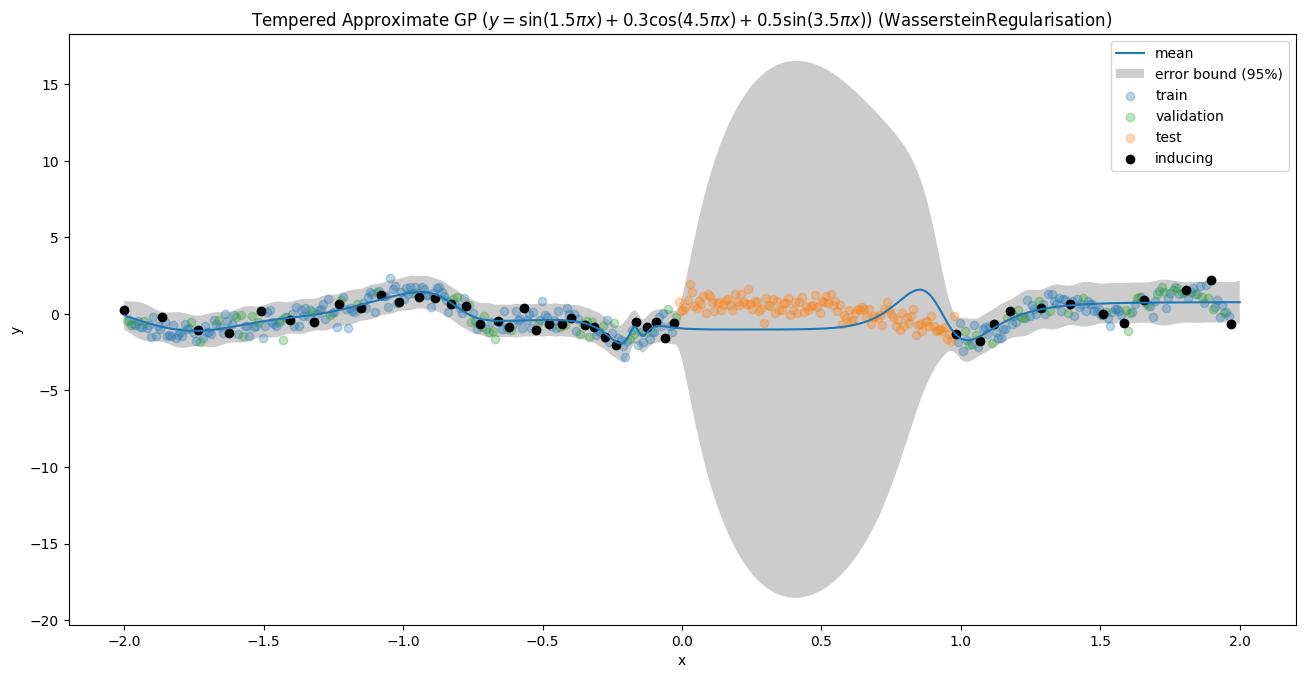
\includegraphics[width=0.9\linewidth]{experiments/regression/toy_curves/outputs/curve3/tempered-WassersteinRegularisation.png}
\end{minipage}%
\begin{minipage}{.5\textwidth}
  \centering
  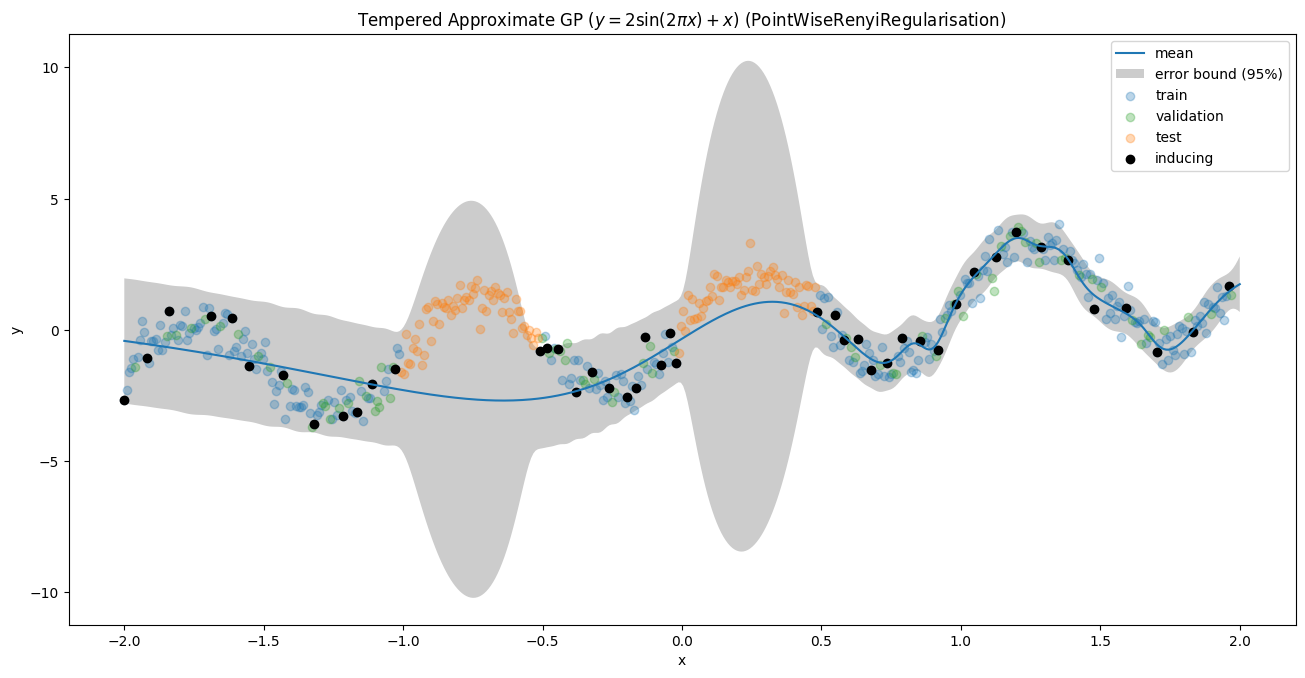
\includegraphics[width=0.9\linewidth]{experiments/regression/toy_curves/outputs/curve4/tempered-PointWiseRenyiRegularisation.png}
\end{minipage}
\caption{GVI-GPs for Regression}
\end{figure}

\subsection{Image Classification}

\newpage
\section{Future Work}
\subsection{NLP Named-Entity Recognition}

\newpage
\section{Conclusions}

\newpage
\bibliography{references}


\newpage
\appendix
\section{Appendix}

\subsection{KL Divergence and the Bayesian Posterior}\label{svgp-kld-bayesian}
We wish to match the log-likelihood of $P_{GP}$ for training data $\left\{ x_n, y_n\right\}$ by maximising the lower bound with respect to $\nu$ for $Q_{GP}^{\nu}$ on inducing points $\{x_m, y_m\}_{m=1}^{M}$. We begin by reformulating the log-likelihood:
\begin{align}
    \mathcal{L} &= \log P\left(\left\{ y_n\right\} \big\vert\left\{ x_n\right\}\right)
    \\&= \log P\left(\left\{ y_n\right\} \big\vert \mathbf{Y}_M, \left\{ x_m\right\}, \left\{ x_n\right\}\right)
    \\&= \log \int_{\mathbb{R}^M} P\left(\left\{ y_n\right\}, \mathbf{Y}_M \big\vert \left\{ x_m\right\}, \left\{ x_n\right\}\right) d\mathbf{Y}_M
\end{align}
Introducing $Q^{\nu}\left(\mathbf{Y}_M \big\vert \left\{ x_m\right\} \right)$, the $Q_{GP}^{\nu}$ prior on the inducing points, we can equivalently write:
\begin{align}
            \mathcal{L} &= \log \int_{\mathbb{R}^M} \frac{P\left(\left\{ y_n\right\}, \mathbf{Y}_M \big\vert \left\{ x_m\right\}, \left\{ x_n\right\}\right)Q^{\nu}\left(\mathbf{Y}_M \big\vert \left\{ x_m\right\} \right)}{Q^{\nu}\left(\mathbf{Y}_M \big\vert \left\{ x_m\right\} \right)} d\mathbf{Y}_M
    \\&= \log \int_{\mathbb{R}^M} \frac{P\left(\left\{ y_n\right\} \big\vert \mathbf{Y}_M , \left\{ x_m\right\}, \left\{ x_n\right\}\right)P\left(\mathbf{Y}_M \big\vert \left\{ x_m\right\}\right)Q^{\nu}\left(\mathbf{Y}_M \big\vert \left\{ x_m\right\} \right)}{Q^{\nu}\left(\mathbf{Y}_M \big\vert \left\{ x_m\right\} \right)} d\mathbf{Y}_M
    \\&\qquad\geq  \int_{\mathbb{R}^M} Q^{\nu}\left(\mathbf{Y}_M \big\vert \left\{ x_m\right\} \right) \log \left(\frac{P\left(\left\{ y_n\right\} \big\vert \mathbf{Y}_M , \left\{ x_m\right\}, \left\{ x_n\right\}\right)P\left(\mathbf{Y}_M \big\vert \left\{ x_m\right\}\right)}{Q^{\nu}\left(\mathbf{Y}_M \big\vert \left\{ x_m\right\} \right)} \right)d\mathbf{Y}_M
    \label{log-like-jensen}
    \\ & \qquad\qquad \eqqcolon \mathcal{F(\nu)}
\end{align}
where we lower bound the log-likelihood with Jensen's inequality in (\ref{log-like-jensen}). $\mathcal{F(\nu)}$ is the free energy or evidence lower bound (ELBO) and can be expressed:
\begin{multline}
    \mathcal{F(\nu)} = \int_{\mathbb{R}^M} Q^{\nu}\left(\mathbf{Y}_M \big\vert \left\{ x_m\right\} \right) \log P\left(\left\{ y_n\right\} \big\vert \mathbf{Y}_M , \left\{ x_m\right\}, \left\{ x_n\right\}\right)d\mathbf{Y}_M
    \\ + \int_{\mathbb{R}^M} Q^{\nu}\left(\mathbf{Y}_M \big\vert \left\{ x_m\right\} \right) \log \left(\frac{P\left(\mathbf{Y}_M \big\vert \left\{ x_m\right\}\right)}{Q^{\nu}\left(\mathbf{Y}_M \big\vert \left\{ x_m\right\} \right)} \right)d\mathbf{Y}_M
\end{multline}
Recovering the standard result:
\begin{align}
    \mathcal{F(\nu)} &=  \log P\left(\left\{ y_n\right\} \big\vert \left\{ x_n\right\}\right) - \KLD\left[Q^{\nu}\left(\mathbf{Y}_M \big\vert \left\{ x_m\right\} \right) \| P\left(\mathbf{Y}_M \big\vert \left\{ x_m\right\} \right)\right]
    \\ &= \sum_{n=1}^N \left[\log P \left(y_n \big\vert  x_n \right)\right] - \KLD\left[Q^{\nu}\left(\mathbf{Y}_M \vert \left\{ x_m\right\} \right) \| P\left(\mathbf{Y}_M \big\vert \left\{ x_m\right\} \right)\right]
\end{align}
We see from (\ref{log-like-jensen}) that $\mathcal{F(\nu)}$ can also be expressed:
\begin{align}
    \mathcal{F(\nu)} &= - \mathbb{E}_{\mathbf{Y}_M \sim Q^{\nu}\left(\mathbf{Y}_M \big\vert \left\{ x_m\right\} \right)} \left[\log \left(\frac{Q^{\nu}\left(\mathbf{Y}_M \big\vert \left\{ x_m\right\} \right)}{P\left(\left\{ y_n\right\} \big\vert \mathbf{Y}_M , \left\{ x_m\right\}, \left\{ x_n\right\}\right)P\left(\mathbf{Y}_M \big\vert \left\{ x_m\right\}\right)} \right) \right]\\
    &= -\KLD \left[Q^{\nu}\left(\mathbf{Y}_M \big\vert \left\{ x_m\right\} \right) \| P\left(\mathbf{Y}_M \big\vert \left\{ x_m\right\}, \left\{ y_n\right\}, \left\{ x_n\right\}\right) \right]
    \label{free-energy-kld}
\end{align}
where we see that $P\left(\mathbf{Y}_M \big\vert \left\{ x_m\right\}, \left\{ y_n\right\}, \left\{ x_n\right\}\right) \propto P\left(\left\{ y_n\right\} \big\vert \mathbf{Y}_M , \left\{ x_m\right\}, \left\{ x_n\right\}\right)P\left(\mathbf{Y}_M \big\vert \left\{ x_m\right\}\right)$, the posterior distribution.
Thus, the KL-divergence is the natural divergence that arises from a Bayesian approach. (\ref{free-energy-kld}) is the negative KL between the prior of the approximating distribution $Q^{\nu}$ and the \textit{true} Bayesian posterior of $P$. In other words, $Q^{\nu*}$ is the projection of the Bayesian posterior onto the space of approximating GPs $\left\{Q^{\nu}: \nu \in \Gamma\right\}$ with respect to the KL-divergence. This is indicated as the minimisation of the $\KLD$ in (\ref{svgp-minimiser}).

\subsection{Trace Kernel Proof for the NNGP Kernel}\label{svgp-kld-bayesian}
\end{document}